\documentclass{standalone}
\usepackage{tikz}
\usetikzlibrary{patterns, positioning}


\begin{document}
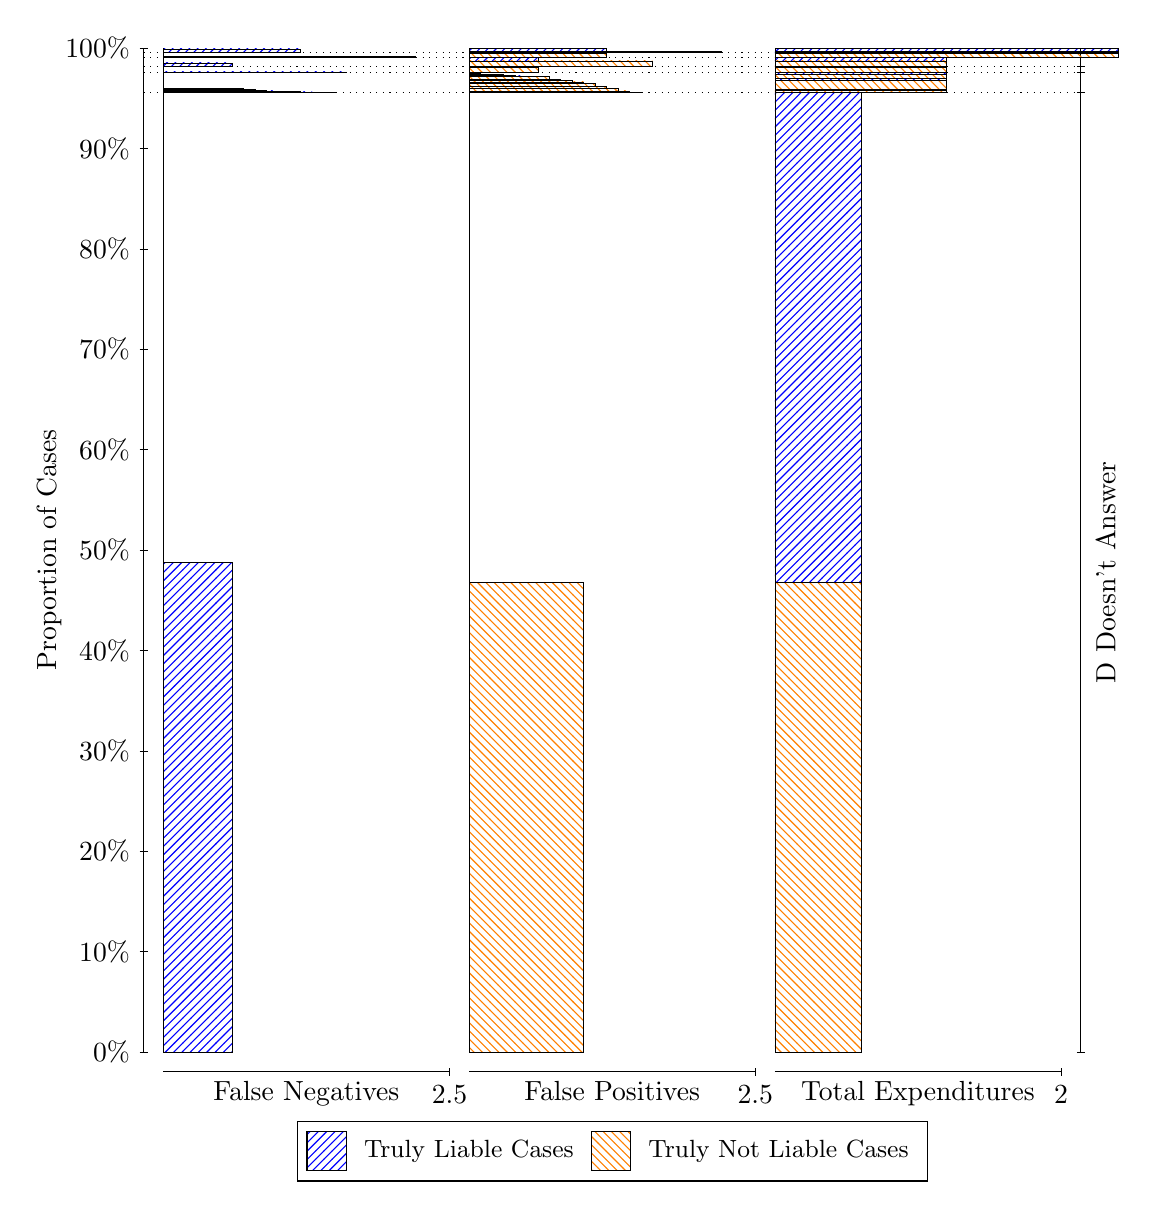
\begin{tikzpicture}
\draw[black, very thin] (1.5,1.75) -- (1.5,14.5);
\node[rotate=90, text=black, anchor=center] at (0.3, 8.125) {Proportion of Cases};
\draw[black, very thin] (1.45,1.75) -- (1.55,1.75);
\node[text=black, anchor=east] at (1.45, 1.75) {0\%};
\draw[black, very thin] (1.45,3.025) -- (1.55,3.025);
\node[text=black, anchor=east] at (1.45, 3.025) {10\%};
\draw[black, very thin] (1.45,4.3) -- (1.55,4.3);
\node[text=black, anchor=east] at (1.45, 4.3) {20\%};
\draw[black, very thin] (1.45,5.575) -- (1.55,5.575);
\node[text=black, anchor=east] at (1.45, 5.575) {30\%};
\draw[black, very thin] (1.45,6.85) -- (1.55,6.85);
\node[text=black, anchor=east] at (1.45, 6.85) {40\%};
\draw[black, very thin] (1.45,8.125) -- (1.55,8.125);
\node[text=black, anchor=east] at (1.45, 8.125) {50\%};
\draw[black, very thin] (1.45,9.4) -- (1.55,9.4);
\node[text=black, anchor=east] at (1.45, 9.4) {60\%};
\draw[black, very thin] (1.45,10.675) -- (1.55,10.675);
\node[text=black, anchor=east] at (1.45, 10.675) {70\%};
\draw[black, very thin] (1.45,11.95) -- (1.55,11.95);
\node[text=black, anchor=east] at (1.45, 11.95) {80\%};
\draw[black, very thin] (1.45,13.225) -- (1.55,13.225);
\node[text=black, anchor=east] at (1.45, 13.225) {90\%};
\draw[black, very thin] (1.45,14.5) -- (1.55,14.5);
\node[text=black, anchor=east] at (1.45, 14.5) {100\%};

\draw[black, very thin] (13.4,1.75) -- (13.4,14.5);
\draw[black, very thin] (13.35,1.75) -- (13.45,1.75);
\node[anchor=west] at (13.35, 1.75) {};
\draw[black, very thin] (13.35,13.932) -- (13.45,13.932);
\node[anchor=west] at (13.35, 13.932) {};
\draw[black, very thin] (13.35,14.187) -- (13.45,14.187);
\node[anchor=west] at (13.35, 14.187) {};
\draw[black, very thin] (13.35,14.269) -- (13.45,14.269);
\node[anchor=west] at (13.35, 14.269) {};
\draw[black, very thin] (13.35,14.38) -- (13.45,14.38);
\node[anchor=west] at (13.35, 14.38) {};
\draw[black, very thin] (13.35,14.448) -- (13.45,14.448);
\node[anchor=west] at (13.35, 14.448) {};
\draw[black, very thin] (13.35,14.5) -- (13.45,14.5);
\node[anchor=west] at (13.35, 14.5) {};

\draw[black, very thin, pattern color=blue, pattern=north east lines] (1.75,1.75) rectangle (2.622,7.9693);
\draw[black, very thin, pattern color=orange, pattern=north west lines] (1.75,7.9693) rectangle (1.75,13.932);
\draw[black, very thin, pattern color=blue, pattern=north east lines] (1.75,13.932) rectangle (3.93,13.937);
\draw[black, very thin, pattern color=blue, pattern=north east lines] (1.75,13.937) rectangle (3.7847,13.939);
\draw[black, very thin, pattern color=blue, pattern=north east lines] (1.75,13.939) rectangle (3.6393,13.942);
\draw[black, very thin, pattern color=blue, pattern=north east lines] (1.75,13.942) rectangle (3.494,13.945);
\draw[black, very thin, pattern color=blue, pattern=north east lines] (1.75,13.945) rectangle (3.3487,13.951);
\draw[black, very thin, pattern color=blue, pattern=north east lines] (1.75,13.951) rectangle (3.2033,13.955);
\draw[black, very thin, pattern color=blue, pattern=north east lines] (1.75,13.955) rectangle (3.058,13.965);
\draw[black, very thin, pattern color=blue, pattern=north east lines] (1.75,13.965) rectangle (2.9127,13.973);
\draw[black, very thin, pattern color=blue, pattern=north east lines] (1.75,13.973) rectangle (2.7673,13.983);
\draw[black, very thin, pattern color=orange, pattern=north west lines] (1.75,13.983) rectangle (1.75,14.187);
\draw[black, very thin, pattern color=blue, pattern=north east lines] (1.75,14.187) rectangle (4.0753,14.197);
\draw[black, very thin, pattern color=orange, pattern=north west lines] (1.75,14.197) rectangle (1.75,14.269);
\draw[black, very thin, pattern color=blue, pattern=north east lines] (1.75,14.269) rectangle (2.622,14.311);
\draw[black, very thin, pattern color=orange, pattern=north west lines] (1.75,14.311) rectangle (1.75,14.38);
\draw[black, very thin, pattern color=blue, pattern=north east lines] (1.75,14.38) rectangle (4.9473,14.392);
\draw[black, very thin, pattern color=orange, pattern=north west lines] (1.75,14.392) rectangle (1.75,14.448);
\draw[black, very thin, pattern color=blue, pattern=north east lines] (1.75,14.448) rectangle (3.494,14.489);
\draw[black, very thin, pattern color=orange, pattern=north west lines] (1.75,14.489) rectangle (1.75,14.5);
\draw[black, very thin, pattern color=orange, pattern=north west lines] (5.6333,1.75) rectangle (7.0867,7.7132);
\draw[black, very thin, pattern color=blue, pattern=north east lines] (5.6333,7.7132) rectangle (5.6333,13.932);
\draw[black, very thin, pattern color=orange, pattern=north west lines] (5.6333,13.932) rectangle (7.8133,13.941);
\draw[black, very thin, pattern color=orange, pattern=north west lines] (5.6333,13.941) rectangle (7.668,13.957);
\draw[black, very thin, pattern color=orange, pattern=north west lines] (5.6333,13.957) rectangle (7.5227,13.991);
\draw[black, very thin, pattern color=orange, pattern=north west lines] (5.6333,13.991) rectangle (7.3773,14.016);
\draw[black, very thin, pattern color=orange, pattern=north west lines] (5.6333,14.016) rectangle (7.232,14.052);
\draw[black, very thin, pattern color=orange, pattern=north west lines] (5.6333,14.052) rectangle (7.0867,14.071);
\draw[black, very thin, pattern color=orange, pattern=north west lines] (5.6333,14.071) rectangle (6.9413,14.09);
\draw[black, very thin, pattern color=orange, pattern=north west lines] (5.6333,14.09) rectangle (6.796,14.103);
\draw[black, very thin, pattern color=orange, pattern=north west lines] (5.6333,14.103) rectangle (6.6507,14.136);
\draw[black, very thin, pattern color=blue, pattern=north east lines] (5.6333,14.136) rectangle (6.36,14.146);
\draw[black, very thin, pattern color=blue, pattern=north east lines] (5.6333,14.146) rectangle (6.2147,14.154);
\draw[black, very thin, pattern color=blue, pattern=north east lines] (5.6333,14.154) rectangle (6.0693,14.164);
\draw[black, very thin, pattern color=blue, pattern=north east lines] (5.6333,14.164) rectangle (5.924,14.168);
\draw[black, very thin, pattern color=blue, pattern=north east lines] (5.6333,14.168) rectangle (5.7787,14.174);
\draw[black, very thin, pattern color=blue, pattern=north east lines] (5.6333,14.174) rectangle (5.6333,14.187);
\draw[black, very thin, pattern color=orange, pattern=north west lines] (5.6333,14.187) rectangle (6.5053,14.258);
\draw[black, very thin, pattern color=blue, pattern=north east lines] (5.6333,14.258) rectangle (5.6333,14.269);
\draw[black, very thin, pattern color=orange, pattern=north west lines] (5.6333,14.269) rectangle (7.9587,14.338);
\draw[black, very thin, pattern color=blue, pattern=north east lines] (5.6333,14.338) rectangle (6.5053,14.38);
\draw[black, very thin, pattern color=orange, pattern=north west lines] (5.6333,14.38) rectangle (7.3773,14.436);
\draw[black, very thin, pattern color=blue, pattern=north east lines] (5.6333,14.436) rectangle (5.924,14.448);
\draw[black, very thin, pattern color=orange, pattern=north west lines] (5.6333,14.448) rectangle (8.8307,14.459);
\draw[black, very thin, pattern color=blue, pattern=north east lines] (5.6333,14.459) rectangle (7.3773,14.5);
\draw[black, very thin, pattern color=orange, pattern=north west lines] (9.5167,1.75) rectangle (10.607,7.7132);
\draw[black, very thin, pattern color=blue, pattern=north east lines] (9.5167,7.7132) rectangle (10.607,13.932);
\draw[black, very thin, pattern color=orange, pattern=north west lines] (9.5167,13.932) rectangle (11.697,13.969);
\draw[black, very thin, pattern color=blue, pattern=north east lines] (9.5167,13.969) rectangle (11.697,13.975);
\draw[black, very thin, pattern color=orange, pattern=north west lines] (9.5167,13.975) rectangle (11.697,14.092);
\draw[black, very thin, pattern color=blue, pattern=north east lines] (9.5167,14.092) rectangle (11.697,14.118);
\draw[black, very thin, pattern color=orange, pattern=north west lines] (9.5167,14.118) rectangle (11.697,14.168);
\draw[black, very thin, pattern color=blue, pattern=north east lines] (9.5167,14.168) rectangle (11.697,14.187);
\draw[black, very thin, pattern color=orange, pattern=north west lines] (9.5167,14.187) rectangle (11.697,14.258);
\draw[black, very thin, pattern color=blue, pattern=north east lines] (9.5167,14.258) rectangle (11.697,14.269);
\draw[black, very thin, pattern color=orange, pattern=north west lines] (9.5167,14.269) rectangle (11.697,14.338);
\draw[black, very thin, pattern color=blue, pattern=north east lines] (9.5167,14.338) rectangle (11.697,14.38);
\draw[black, very thin, pattern color=orange, pattern=north west lines] (9.5167,14.38) rectangle (13.877,14.436);
\draw[black, very thin, pattern color=blue, pattern=north east lines] (9.5167,14.436) rectangle (13.877,14.448);
\draw[black, very thin, pattern color=orange, pattern=north west lines] (9.5167,14.448) rectangle (13.877,14.459);
\draw[black, very thin, pattern color=blue, pattern=north east lines] (9.5167,14.459) rectangle (13.877,14.5);
\draw[black, dotted] (1.5,13.932) -- (13.4,13.932);
\draw[black, dotted] (1.5,14.187) -- (13.4,14.187);
\draw[black, dotted] (1.5,14.269) -- (13.4,14.269);
\draw[black, dotted] (1.5,14.38) -- (13.4,14.38);
\draw[black, dotted] (1.5,14.448) -- (13.4,14.448);
\draw[black, very thin] (1.75,1.5) -- (5.3833,1.5);
\node[text=black, anchor=north] at (3.5667, 1.5) {False Negatives};
\draw[black, very thin] (5.3833,1.45) -- (5.3833,1.55);
\node[text=black, anchor=north] at (5.3833, 1.45) {2.5};

\draw[black, very thin] (5.6333,1.5) -- (9.2667,1.5);
\node[text=black, anchor=north] at (7.45, 1.5) {False Positives};
\draw[black, very thin] (9.2667,1.45) -- (9.2667,1.55);
\node[text=black, anchor=north] at (9.2667, 1.45) {2.5};

\draw[black, very thin] (9.5167,1.5) -- (13.15,1.5);
\node[text=black, anchor=north] at (11.333, 1.5) {Total Expenditures};
\draw[black, very thin] (13.15,1.45) -- (13.15,1.55);
\node[text=black, anchor=north] at (13.15, 1.45) {2};

\node[text=black, centered, rotate=90] at (13.72, 7.8412) {D Doesn't Answer};






\draw (7.449999999999999,1.5) node[draw=none] (baseCoordinate) {};
\begin{scope}[align=center]
        \matrix[scale=0.5, draw=black, below=0.5cm of baseCoordinate, nodes={draw}, column sep=0.1cm]{
            \node[rectangle, draw, minimum width=0.5cm, minimum height=0.5cm, pattern color=blue, pattern=north east lines] {}; &
            \node[draw=none, font=\small, text=black] (B) {Truly Liable Cases}; &
            \node[rectangle, draw, minimum width=0.5cm, minimum height=0.5cm, pattern color=orange, pattern=north west lines] {}; &
            \node[draw=none, font=\small, text=black] (B) {Truly Not Liable Cases}; \\
            };
\end{scope}

\end{tikzpicture}
\end{document}